\par Para esta etapa se busca calcular los tiempos de reverberación óptimos y diseñar el tratamiento acústico de la sala, teniendo en cuenta que la misma va a ser utilizada para palabra. Dicho tratamiento consta de la utilización de materiales fonoabsorbentes en paredes y asientos.\\

\par Para realizar este tratamiento, comezamos calculando el tiempo de reverberación ($TR$) óptimo considerando el volumen de la sala y el uso que se le dará a la misma (en nuestro caso, la palabra). Utilizando las curvas de \quotemarks{TR óptimos según el volumen y destino de uso} de \textit{Knudsen}, y gracias a las fórmulas provistas por la cátedra que modelan dichas curvas, podemos calcular los tiempos de reverberación óptimos presentes en el cuadro~\tableref{tab:ecuaciones_caluclo_TRoptimo} :

\begin{table}[h]
    \centering
    \begin{tabular}{|c|c|} \hline
        \textbf{Frecuencia [Hz]}  & \textbf{$TR_{opt}(V)$ [seg]}; V en $m^3$\\ \hline
        125 & $TR_{125} = 0.41 + 0.26 \cdot log(V)$ \\ \hline
        250 & $TR_{250} = 0.32 + 0.21 \cdot log(V)$ \\ \hline
        >500 & $TR_{500} = 0.28 + 0.18 \cdot log(V)$ \\ \hline
    \end{tabular}
    \caption{Ecuaciones para cálculo de $TR_{optimos}$}
    \label{tab:ecuaciones_caluclo_TRoptimo}
\end{table}

\par A partir del volumen resultante de la sala, $V = 354.45 m^3$, se obtiene el cuadro~\tableref{tab:medidas_de_sala}. Por lo tanto, los $TR_{optimos}$ obtenidos se presentan en el cuadro~\tableref{tab:TRoptimos_de_sala}. Como criterio de diseño, debemos considerar una banda de tolerancia para los valores obtenidos. Consideramos prudente una banda de tolerancia del 20\%. Dichos valores fueron redondeados a 1 decimal, debido a que no podemos asegurar mayor precisión con la aproximación utilizada.

\begin{table}[h]
    \centering
    \begin{tabular}{|c|c|} \hline
         $TR_{optimos}$ [seg] & $\Delta TR$ [seg] \\ \hline 
         $TR_{125} = 1.1$  & $0.2$ \\ \hline
         $TR_{250} = 0.9$  & $0.2$\\ \hline
         $TR_{500} = 0.7$  & $0.1$ \\ \hline
    \end{tabular}
    \caption{Tiempos de reverberación óptimos para uso de Palabra para la sala estudiada}
    \label{tab:TRoptimos_de_sala}
\end{table}

\par En la figura~\figref{fig:TR_optimosYtolerancia} se muestran los valores obtenidos junto con sus bandas de tolerancia para frecuencias de octavas comprendidas entre 125 y 4000Hz.


\begin{figure}[H]
	\centering
	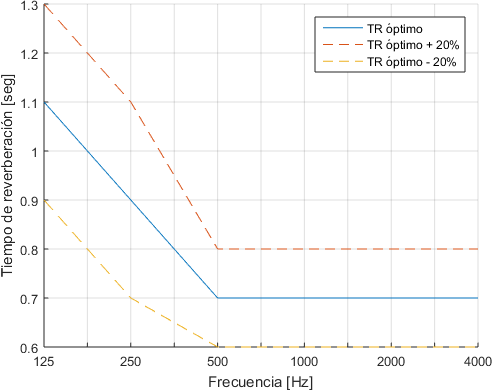
\includegraphics[width=1\textwidth]{./img/TR_optimosYtolerancia.png}
	\caption{Gráfico de valores de $TR_{optimo}$ y sus bandas de tolerancia}
	\label{fig:TR_optimosYtolerancia}
\end{figure}

\par A continuación, seleccionamos los materiales con que estarán construidas las superficies interiores del recinto (piso, techo, paredes, puertas) y la cantidad de muebles. Para esto, consideramos las recomendaciones de diseño acústico para aulas y salas de conferencias del \quotemarks{\textit{Código Técnico de la Edificación}} (\textbf{CTE} España), donde se recomienda material absorbente acústico en toda la superficie del techo, una pared detrás del orador reflectante y las demás absorbentes. Los materiales para el recinto se muestran en el cuadro~\tableref{tab:materiales_construccion_recinto}.

\hfill

\clearpage

\begin{table}[H]
    \centering
    \begin{tabular}{|c|c|c||c|c|c|c|c|c|} \hline
        Tipo &  Material elegido &Sup./Cant. & \multicolumn{6}{|c|}{Coeficiente $\alpha$ / Área equivalente [$m^2$]} \\ \hline
        \multicolumn{3}{|c|}{Frecuencia [Hz]:} & 125 & 250 & 500 & 1000 & 2000 & 4000 \\ \hline \hline
        Piso & Baldosa enlozada & 104.25$m^2$ & 0.01 & 0.02 & 0.02 & 0.03 & 0.03 & 0.04 \\ \hline
        Techo & Hormigón & 104.25$m^2$ & 0.01 & 0.01 & 0.02 & 0.02 & 0.05 & 0.07 \\ \hline
        Paredes (frente orador) & Papel Pintado & 89.26 $m^2$ & 0.01 & 0.20 & 0.04 & 0.10 & 0.20 & 0.30 \\ \hline
        Pared (detrás orador) & Ladrillo pintado & 47.26 $m^2$ & 0.01 & 0.01 & 0.02 & 0.02 & 0.02 & 0.02 \\ \hline
        Puertas (1.5m x 2m) & Madera maciza & 3 $\times$ 3$m^2$ & 0.05 & 0.11 & 0.10 & 0.09 & 0.08 &  0.10 \\ \hline \hline
        Butacas & Tapizado 1 & 120 Unid. & 0.12 & 0.20 & 0.28 & 0.30 & 0.31 & 0.37 \\ \hline
        Butaca & Madera & 1 Unid. & 0.01 & 0.02 & 0.02 & 0.04 & 0.04 & 0.04 \\ \hline
    \end{tabular}
    \caption{Materiales y objetos para la construcción del recinto}
    \label{tab:materiales_construccion_recinto}
\end{table}

\par En donde:

\begin{itemize}
    \item La superficie del piso se calcula: $S_{piso} = L \cdot W = 13.9 \cdot 7.5m^2 = 104.25m^2$
    \item La superficie del techo es la misma que la del piso, por lo tanto $S_{techo} = 104.25m^2$
    \item La superficie de las 3 paredes que se encuentran al frente del orador se calculan: $S_{frenteOrador} = H \cdot L + H \cdot W \cdot 2 - S_{puertas} = 3.4 \cdot 13.9 m^2+ 3.4 \cdot 7.5 \cdot 2 m^2 - 3 \cdot 3m^2 = 89.26m^2$
    \item La superficie de la pared detrás del orador: $S_{detrasOrador} = H \cdot L = 3.4 \cdot 13.9 m^2 = 47.26m^2$
    \item La superficie que cubren las puertas de madera se calculan sabiendo que las mismas son 3 y cada una cubre $3m^2$
    \item Para las butacas, tenemos 120 unidades de las butacas con tapizado tipo 1 y 1 butaca de madera para el presentador
\end{itemize}

%\par Para las paredes hacia donde el orador expone, la recomendación indica que deben colocarse materiales absorbentes, por lo tanto, se optó por papel pintado, cuyos coeficientes de absorción sonora son más altos que los de los demás materiales. Tanto para el piso y techo se utilizó un criterio semejante, es decir, se consideró un material que se caracterice por tener coeficientes de absorción altos sin que afecte las curvas en altas frecuencias. Así es como se seleccionó la baldoza enlozada para el piso y enlucido para el techo. Luego, como buscabamos una pared reflejante detrás del orador, se optó por construir dicha superficie con ladrillo pintado.

\par A partir de la elección de los materiales, se esperá cumplir con los tiempos de reverberación óptimos para una  \textcolor{red}{ocupación del \textbf{75\%}}. En caso de no cumplirlo, se realizará un tratamiento acústico a la sala.\\

\par A continuación, procedemos a calcular el tiempo de reverberación inicial correspondiente a la sala equipada con los elementos y muebles elegidos, para tener una noción inicial que sirva de referencia. Para esto, utilizamos la ecuación~\eqref{eq:Calculo_tiempo_reverberacion}, a partir de la cual se puede  calcular el tiempo de reverberación, la cuál considera el área equivalente resultante.

\begin{equation}
   \mathcolorbox{EQColor}{  TR = \frac{0.163 \cdot V}{A_T} }
    \label{eq:Calculo_tiempo_reverberacion}
\end{equation}

Donde:
\begin{itemize}
    \item $V$: Es el volumen de la sala en $m^3$
    \item $A_T$: Es el área equivalente de absorción total en el recinto, expresado en $m^2$
\end{itemize}

\par Para utilizarla, es necesario obtener la expresión de $A$. Primero, calculamos el área equivalente del local sin muebles ni personas, $A_L$, mediante la siguiente expresión:

\begin{equation}
    A_L = S_{piso} * \alpha_{piso} +S_{techo} * \alpha_{techo} + S_{pared} * \alpha_{pared} + S_{puertas} * \alpha_{puertas}
\end{equation}

\par Donde, $S_i$ corresponde a las múltiples superficies presentes en la sala y $\alpha_i$, corresponde al coeficiente de absorción asociado a cada material. Estos últimos son datos extraidos de la guía de materiales utilizada para el trabajo.

\par Como segunda instancia, incorporamos los muebles elegidos. Entonces, a la ecuación previa, le sumamos el área equivalente de las butacas a instalar y multiplicamos por la cantidad  utilizada:

\begin{equation}
    A_1 = A_L + n_{Butacas}\cdot A_{Butacas}
\end{equation}

\par Luego, considerando el efecto que tienen las personas dentro del recinto, y asumiendo que las butacas se ocupan un 75\%. De acuerdo al tipo de butacas elegido, tapizada tipo 1, el área equivalente de absorción sonora provocado por un adulto en dicha butaca, surge de la expresión:

\begin{equation}
    A_2 = A_L + n_{ButacasVacias} \cdot A_{Butacas} + n_{ButacasOcupadas} \cdot A_{ButacasOcupadas}
\end{equation}

\par Dadas estas consideraciones, obtenemos la figura~\figref{fig:TR_conPersonas} y el cuadro~\figref{tab:TR_conPersonas} como resultado:

\begin{figure}[H]
	\centering
	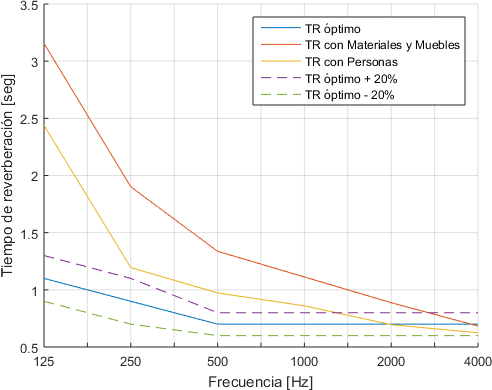
\includegraphics[width=1\textwidth]{./img/TR_conMat_MueblesYPersonas.png}
	\caption{Curvas de $TR_{optimo}$ comparados con la sala ocupada al 75\%, con muebles y materiales}
	\label{fig:TR_conPersonas}
\end{figure}

\begin{table}[H]
    \centering
    \begin{tabular}{|c|c|c|c|c|c|} \hline
        Frec. [Hz] &$TR_{optimo}(-20\%)$& $TR_{optimo}$ & $TR_{optimo}(+20\%)$  & $TR_{SinPersonas}$ & $TR_{ConPersonas}$ \\  \hline
        125 & 0.9 seg & 1.1 seg & 1.3 seg & 2.44 seg & 3.16 seg \\ \hline
        250 & 0.7 seg & 0.9 seg & 1.1 seg & 1.19 seg & 1.90 seg \\ \hline
        500 & 0.6 seg & 0.7 seg & 0.8 seg & 0.97 seg & 1.34 seg \\ \hline
        1k & 0.6 seg & 0.7 seg & 0.8 seg & 0.86 seg & 1.11 seg \\ \hline
        2k & 0.6 seg & 0.7 seg & 0.8 seg & 0.70 seg & 0.89 seg \\ \hline
        4k & 0.6 seg & 0.7 seg & 0.8 seg & 0.62 seg & 0.68 seg \\ \hline
    \end{tabular}
    \caption{Valores de $TR_{optimo}$ comparados con la sala ocupada al 75\%, con materiales y muebles}
    \label{tab:TR_conPersonas}
\end{table}


\par Observamos que aún considerando el efecto de las personas en la sala, se necesita un tratamiento fonoabsorbente. Observamos que es necesario bajar los valores de tiempo de reverberación para las frecuencias mas bajas y bajar las frecuencias altas a menor medida. Para esto, se considera la recomendación de diseño que indica colocar materiales fonoabsorbentes en el las paredes opuestas al orador y en el techo, mientras que la pared detrás de este, sea de un material reflejante (es por eso que se optó Ladrillo pintado para la pared detrás del orador, que tiene bajos valores de $\alpha$). Por lo tanto se resolvio colocar paneles de madera, aglomerado 6 mm, sobre 50 mm lana de vidrio en el 40\% de la superficia de las paredes que se encuentran frente al orador, y en el caso del techo, se decidió cubrirlo un 10\% con cielorraso 4, el cuál consta de un panel yeso acanalado $+$ lana 50mm, 35 kg/m² $+$ 85 cm aire. Dichos materiales poseen las características que se indican en el cuadro~\tableref{tab:datos_mat_fonoabsorbente}.

\begin{table}[h]
    \centering
    \begin{tabular}{|c|c|c||c|c|c|c|c|c|} \hline
         Material Elegido & Sup. & \multicolumn{6}{|c|}{Coeficiente $\alpha$} \\ \hline
        \multicolumn{2}{|c|}{Frecuencia [Hz]:} & 125 & 250 & 500 & 1000 & 2000 & 4000 \\ \hline
        \makecell{Panel madera, aglomerado 6 mm,\\ sobre 50 mm lana de vidrio} & 35.70$m^2$ & 0.61 &0.65&0.24&0.12&0.10&0.06 \\ \hline  
        \makecell{Cielorraso 4: Panel yeso acanalado $+$\\ lana 50mm, 35 kg/m² + 85 cm aire} & 10.43$m^2$ & 0.56 & 0.60 & 1.00 & 0.83 & 0.49 & 0.31 \\ \hline
    \end{tabular}
    \caption{Material fonoabsorbente elegido}
    \label{tab:datos_mat_fonoabsorbente}
\end{table}

\par En donde:
\begin{itemize}
    \item La superficie cubierta por el panel de madera en la pared se calcula como: $S_{PanelMadera} = S_{FrenteOrador} \cdot 0.4 = 89.26m^2 \cdot 0.4= 35.70m^2$
    \item La superficie cubierta por el panel de Yeso en el techo se calcula como: $S_{PanelYeso} = S_{Techo} \cdot 0.1 = 104.25 m^2 \cdot 0.1 = 10.43m^2$
\end{itemize}

\par Finalmente, volvemos a calcular el tiempo de reverberación considerando los cambios del fonoabsorbente elegido mediante:

\begin{align*}
        A_T &= A_2 - (0.4 \cdot S_{ParedFrenteOrador} * \alpha_{ParedFrenteOrador}) + (0.4 \cdot S_{ParedFrenteOrador} * \alpha_{PanelMadera})\\
    &\quad -(0.1 \cdot S_{Techo} * \alpha_{Techo}) + (0.1 \cdot S_{Techo} * \alpha_{PanelYeso})
\end{align*}


\par Obteniendose la figura~\figref{fig:TR_fonoabsorbente} y el cuadro~\figref{tab:TR_fonoabsorbente} :

\begin{figure}[H]
	\centering
	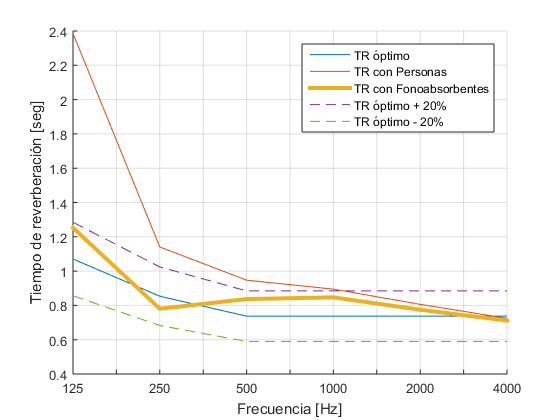
\includegraphics[width=1\textwidth]{./img/TR_conFonoabsorbentes.png}
	\caption{Curvas de $TR_{optimo}$ comparados con la sala ocupada al 75\%, solo con materiales y muebles, y con los materiales fonoabsorbentes}
	\label{fig:TR_fonoabsorbente}
\end{figure}

\begin{table}[H]
    \centering
    \begin{tabular}{|c|c|c|c|c|c|} \hline
        Frec. [Hz] &$TR_{optimo}(-20\%)$& $TR_{optimo}$ & \textcolor{green}{$TR_{conFonoabsorbente}$}& $TR_{optimo}(+20\%)$  \\  \hline
        125 & 0.9 seg & 1.1 seg& 1.10 seg & 1.3 seg  \\ \hline
        250 & 0.7 seg & 0.9 seg& 0.75 seg & 1.1 seg  \\ \hline
        500 & 0.6 seg & 0.7 seg& 0.75 seg & 0.8 seg  \\ \hline
        1k & 0.6 seg & 0.7 seg & 0.76 seg & 0.8 seg  \\ \hline
        2k & 0.6 seg & 0.7 seg & 0.69 seg &0.8 seg  \\ \hline
        4k & 0.6 seg & 0.7 seg & 0.67 seg& 0.8 seg  \\ \hline
    \end{tabular}
    \caption{Valores de $TR_{optimo}$ comparados con la sala ocupada al 75\%, solo con materiales y muebles, y con los materiales fonoabsorbentes}
    \label{tab:TR_fonoabsorbente}
\end{table}

\par Dada la figura previa, observamos que la curva de $TR$ con el recinto tratado con fonoabsorbentes se mantiene dentro de los límites de tolerancia considerados.

\par Dado esto, pasamos a calcular la inteligibilidad de la palabra dentro del recinto. Sabemos que una palabra consta de vocales y consonantes. La comprensión de un mensaje oral depende fundamentalmente de la correcta percepción de sus consonantes, por lo tanto es de vital importancia percibir bien las altas frecuencias.

\par En el cuadro~\tableref{tab:Contribucion_inteligibilidad_x_banda_de_octava} podemos observar una clasificación, en bandas de octavas, de la contribución de las frecuencias a la inteligibilidad de la palabra y al nivel sonoro. En ella se aprecia que las frecuencias de la octava centrada en 2 kHz son las que tienen mayor influencia en la inteligibilidad de la palabra. Por este motivo en la práctica, se suelen hacer los cálculos para 2 kHz.

\begin{table}[h]
    \centering
    \begin{tabular}{|c|c|c|c|c|c|} \hline
        Frecuencias [Hz] & 250 & 500 & 1k & 2k & 4k  \\ \hline
        Nivel sonoro &22\%& 46\% & 20\% &3\% &2\% \\ \hline
        Inteligibilidad &5\% &13\% &20\% &31\% &26\% \\ \hline
    \end{tabular}
    \caption{Contribución de la inteligibilidad de la palabra para cada banda de octava}
    \label{tab:Contribucion_inteligibilidad_x_banda_de_octava}
\end{table}

\par Para evaluar la inteligibilidad hay varios métodos, de los cuales, uno de los más difundidos es el que se basa en el estudio de la pérdida real de consonantes.

\par En una sala que tiene un valor bajo de \%Alcons (\textit{Articulation Loss of Consonants} ó Pérdida de consonantes) es más sencillo entenderse que en una que tiene un valor alto de \%Alcons. El valor se basa exclusivamente en el porcentaje de consonantes medio que no pueden llegar a entender los oyentes de una sala, ya que las vocales no son tan necesarias para entender un mensaje.

\par Existe un modelo matemático para el cálculo de dicho valor utilizando uso de la teoría acústica estadística. Peutz dedujo el valor de \%Alcons como la diferencia entre los niveles sonoros de campo directo y de campo reverberante. La ecuación~\eqref{eq:diferencia_L_D_LR} muestra el cálculo de dicho valor el cuál debe interpretarse como la relación señal/ruido en lo que respecta la comprensión del lenguaje.

\begin{equation}
   \mathcolorbox{EQColor}{ L_D - L_R = 10 \cdot log \left(\frac{Q \cdot R}{ d^2} \right) - 17dB }
    \label{eq:diferencia_L_D_LR}
\end{equation}
%Me dio -11.22 dB

\par En donde:
\begin{itemize}
    \item $Q$: El factor de directividad de la fuente sonora en la dirección considerada (Q = 2 en el caso de la voz humana, considerando la dirección frontal del orador).
    \item $d$: La distancia entre el emisor (orador) y el receptor, en $m$.
    \item $R$: La constante acústica de la sala, en $m^2$
\end{itemize}

\par Recordando que la constante $R$ esta dada por:

\begin{equation}
   \mathcolorbox{EQColor}{ R  = \frac{A}{1- \bar{\alpha}} = \frac{0.161 \cdot V}{T_{60} (1- \bar{\alpha})} }
\end{equation}

\par En donde:
\begin{itemize}
    \item $A$: El área equivalente de absorción sonora de la sala, $m^2$.
    \item $V$: Volumen de la sala, en $m^3$.
    \item $T_{60}$: Tiempo de reverberación de la sala, en $seg$.
    \item $\bar{\alpha}$: Coeficiente medio de absorción de la sala (adimensional).
    \item $S_L$: Superficie interior del local, en $m^2$.
\end{itemize}

\par Con:

\begin{equation}
   \mathcolorbox{EQColor}{ \bar{\alpha} = \frac{\alpha_1 \cdot S_1 + \alpha_2 \cdot S_2 + ... + \alpha_n \cdot S_n}{S_1 +S_2 + ...+ S_n} \approx \frac{A}{S_L} }
\end{equation}

\par Según Peutz, se define el \textit{nivel de inteligibilidad}, IL\% como:

\begin{equation}
   \mathcolorbox{EQColor}{ IL_{\%} = 100 - AL_{\%} }
\end{equation}

\par Y la pérdida de articulación de consonantes \%Alcons:

\begin{equation}
    \mathcolorbox{EQColor}{ AL_{\%} = 9 \cdot T_{60} }
    \label{eq:calculoAlcons}
\end{equation}

\par Dicha ecuación, se utiliza para distancia de público $d>3.16\cdot D_c$, donde $D_c$ es la distancia crítica, en $m$, que se calcula como:

\begin{equation}
   \mathcolorbox{EQColor}{ D_c = 0.06 \cdot \sqrt{\frac{Q \cdot V}{T_{60} (1- \hat{\alpha})}} = 0.15 \cdot \sqrt{Q\cdot R} }
\end{equation}

\par Como los cálculos se realizan para el público que se encuentra a mayor distancia del orador (es decir, 7.5m), estamos utilizando la ecuación de $Alcons_{\%}$ correcta.\\

\par Ahora podemos calcular la inteligibilidad de la palabra utilizando las ecuaciones dadas:

\begin{equation*}
        R  = \frac{0.161 \cdot V}{TR_{2kHz} (1- \bar{\alpha_{2kHz}})} =  \frac{0.161 \cdot 354.45 m^3}{0.6872 seg \cdot (1- 0.2375)} =108.9 m^2
\end{equation*}

\begin{equation*}
        D_c = 0.15 \sqrt{Q\cdot R} = 0.15 \sqrt{ 2\cdot 108.9 m^2} =  2.21m
\end{equation*}

\par Entonces como $D_c \cdot3.16 = 6.99m < d = 7.5m$, podemos decir que utilizamos la correcta expresión de \%Alcons:

\begin{equation*}
   \boxed{ IL_{\%} = 100 - AL_{\%} = 100 - 9\cdot TR_{2kHz} =  93.82\% }
\end{equation*}

\par Entonces \textcolor{red}{ $IL_{\%} =93.82\%$ } $> 90\% $ lo cuál era el objetivo principal del diseño. Por lo tanto se cumple lo pedido.\\

\par Dado que $D_c = 2.21m$, observamos que existen butacas que se encuentran a $1m$ del orador, y en ese caso deberíamos cambiar la expresión~\eqref{eq:calculoAlcons} para calcular la pérdida de consonantes por la expresión~\eqref{eq:calculoAlconsAlternativo}.

\begin{equation}
    \mathcolorbox{EQColor}{ AL_{\%} = \frac{200 \cdot d^2 \cdot TR_{2kHz}^2}{Q\cdot V} }
    \label{eq:calculoAlconsAlternativo}
\end{equation}

Utilizando $d=1m$ obtenemos:

\begin{equation*}
    \boxed{ AL_{\%} = \frac{200 \cdot d^2 \cdot TR_{2kHz}^2}{Q\cdot V} = \frac{200 \cdot 1m^2 \cdot 0.6872 seg^2}{2 \cdot 354.45m^3} = 0.1939 }
\end{equation*}

\par Tendríamos entonces un nivel de inteligibilidad de la palabra de $IL_{\%}$ =  99.81\%. Por lo tanto, no es importante hacer que todas las filas de butacas se encuentren a partir de la distancia crítica para el recinto diseñado. Para verificar, podemos ver en la figura~\figref{fig:nivel_inteligibilidad} un gráfico de la expresión~ \eqref{eq:calculoAlconsAlternativo} en función de la distancia, en el cuál verificamos que el nivel de inteligibilidad se mantiene por encima de 90\% hasta la distancia crítica.

\begin{figure}[H]
	\centering
	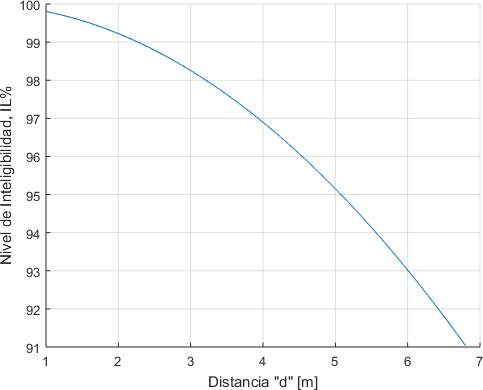
\includegraphics[width=1\textwidth]{./img/nivel_inteligibilidad.png}
	\caption{Inteligibilidad de la palabra en función de la distancia del orador hasta el receptor más cercano}
	\label{fig:nivel_inteligibilidad}
\end{figure}